%!xelatex = 'xelatex --halt-on-error %O %S'

\documentclass{thuemp}
\begin{document}

% 标题,作者
\emptitle{}
\empauthor{王驰}{王合英}

% 奇数页页眉 % 请在这里写出第一作者以及论文题目
\fancyhead[CO]{{\footnotesize 王驰:多晶X射线衍射的物相分析及其应用}}


%%%%%%%%%%%%%%%%%%%%%%%%%%%%%%%%%%%%%%%%%%%%%%%%%%%%%%%%%%%%%%%%
% 关键词 摘要 首页脚注
%%%%%%%%关键词
\Keyword{}
\twocolumn[
\begin{@twocolumnfalse}
\maketitle

%%%%%%%%摘要
\begin{empAbstract}
\end{empAbstract}

%%%%%%%%英文标题、作者、摘要、关键词
\emptitleEn{Experiments of Modern Physics in Tsinghua University}
\empauthorEn{Chi Wang}{Heying Wang}
\KeywordEn{keyword1, keyword2, keyword3, keyword4, keyword5}

\begin{empAbstractEn}
\end{empAbstractEn}

%%%%%%%%首页角注,依次为实验时间、报告时间、学号、email
\empfirstfoot{2024-09-29}{2025-06-09}{2022012259}{chi-wang22@mails.tsinghua.edu.cn}
\end{@twocolumnfalse}
]
%%%%%%%%!首页角注可能与正文重叠,请通过调整正文中第一页的\enlargethispage{-3.3cm}位置手动校准正文底部位置:
%%%%%%%%%%%%%%%%%%%%%%%%%%%%%%%%%%%%%%%%%%%%%%%%%%%%%%%%%%%%%%%%
%  正文由此开始
\wuhao 
%  分栏开始

\section{引言}
\enlargethispage{-3.3cm}

\section{实验内容}

本实验使用X射线衍射仪,对提供的各晶体粉末样品进行X射线衍射分析,测绘出X射线衍射谱,并使用Jade 9软件对所得衍射谱进行寻峰,结合粉末衍射文件(Powder Diffraction File, PDF)卡片进行分析比对,确认物质组成,并利用Nelson-Riley外推法,对晶格常数进行精密测量。

所使用的X射线仪中【如图...】,X射线管以及探测器可相对于样品托架的法向进行对称转动,保持X射线探测方向与入射方向满足平面反射关系;在此过程中,X射线管发射出波长一定的X射线,经过托架上的样品衍射后,部分X射线进入探测器,其强度与衍射角$\theta$关系即被记录下来,形成X射线衍射谱。本实验所采用的X射线管靶材为$\text{Cu}$,使用特征谱线$\text{Cu~K\alpha}$($\lambda = 1.54059~\angstrom$)设置电压$38~\text{kV}$,电流$10~\text{mA}$,在X射线管与探测器夹角$2\theta$取$20^\circ \~ 120^\circ$的区间内,选择步长$0.03^\circ$,对样品X射线衍射谱进行测绘。

本实验所使用的样品中,已知化学组分的有多晶硅粉末($\text{Si}$)、氯化钠粉末($\text{NaCl}$)、氯化钠单晶($\text{Si}$)、铜($\text{Cu}$),钼($\text{Mo}$),石墨烯粉末($\text{C}$)、石墨粉末($\text{C}$)、金刚石粉末($\text{Si}$),另有一份白色粉末状试样化学成分尚待本次实验测定。

\section{实验结果与分析}

\subsection{多晶硅的X射线衍射谱测量}

\subsubsection{多晶硅X射线衍射峰分布的理论分析}

首先对多晶硅X射线衍射峰分布进行分析:在晶体衍射中,对各个晶面以及相应晶面间距$d$,其衍射峰对应衍射角$\theta$满足Bragg公式:

\begin{equation}
    2d\sin\theta  = \lambda
    \label{eq:bragg}
\end{equation}

对于晶体引入晶面常数$(h,k,l)$刻画各个取向以及间隔上的各族晶面。在硅等立方晶系晶体中,记晶格常数为$a$,可以给出相应晶面的间距$d_{hkl}$:

\begin{equation}
    d_{hkl} = \sqrt{h^2+l^2+k^2} a
    \label{eq:d_hkl}
\end{equation}

这也就对应于一系列衍射峰位置$\theta_{hkl}$:

\begin{equation}
    \sin^2 \theta_{hkl} = \frac{\lambda^2}{4a^2}(h^2+k^2+l^2)
    \label{eq:theta_hkl}
\end{equation}

晶面在衍射极大时的衍射强度与晶胞内原子位置有关,表现为受到以下结构因子调制:

\begin{equation}
    F_{hkl} = \sum_{j = 1}^{N} f_j exp{2\pi i (hx_j + ky_j + lz_j)}
    \label{eq:structure_factor}
\end{equation}

其中$f_j$为原子散射因子,$(x_j,y_j,z_j)$为原子坐标。对于硅,其具有金刚石结构(空间群:$Fd\bar{3}m$),晶胞包含8个原子(如图【】),原子分数坐标为:

\begin{align*}
(0,0,0),\quad &(0,\frac{1}{2},\frac{1}{2}),\quad (\frac{1}{2},0,\frac{1}{2}),\quad (\frac{1}{2},\frac{1}{2},0) \\
(\frac{1}{4},\frac{1}{4},\frac{1}{4}),\quad &(\frac{1}{4},\frac{3}{4},\frac{3}{4}),\quad (\frac{3}{4},\frac{1}{4},\frac{3}{4}),\quad (\frac{3}{4},\frac{3}{4},\frac{1}{4})
\end{align*}

代入计算,得到结构因子:

\begin{equation}
    F_{hkl}^{\text{Si}} = f_{Si} \left[1 + e^{\pi i (h+k)} + e^{\pi i (h+l)} + e^{\pi i (k+l)}\right]
    \label{eq:si_struct_fac}
\end{equation}

这就给出其消光特性:

\begin{itemize}
    \item \textbf{全奇或全偶数}:$h,k,l$全为奇数或全为偶数时(以下均假定$h,k,l \in \mathbb{N}$)
    \begin{itemize}
    \end{itemize}
    \item \textbf{混合奇偶}:$h,k,l$奇偶混合时$F_{hkl}=0$(消光)
\end{itemize}

由此可知$(111), (220), (311), (400), (331)$等晶面可观测衍射峰,而$(100), (110), (210)$等因消光不可见。这在衍射峰的分布上就表现为:

\begin{equation}
    \sin{\theta_1} : \sin{\theta_2} :\sin{\theta_3} : \sin{\theta_4} : \cdots = 
    : : : : : \cdots
\label{eq:si_diff_patt}
\end{equation}

\subsubsection{多晶硅X射线衍射实验数据对比}

在$2\theta$取$20.0^\circ \sim 120.0^\circ$范围内进行扫描,得到谱图以及Jade软件寻峰结果如下:

\begin{figure}[H]
    \centering
    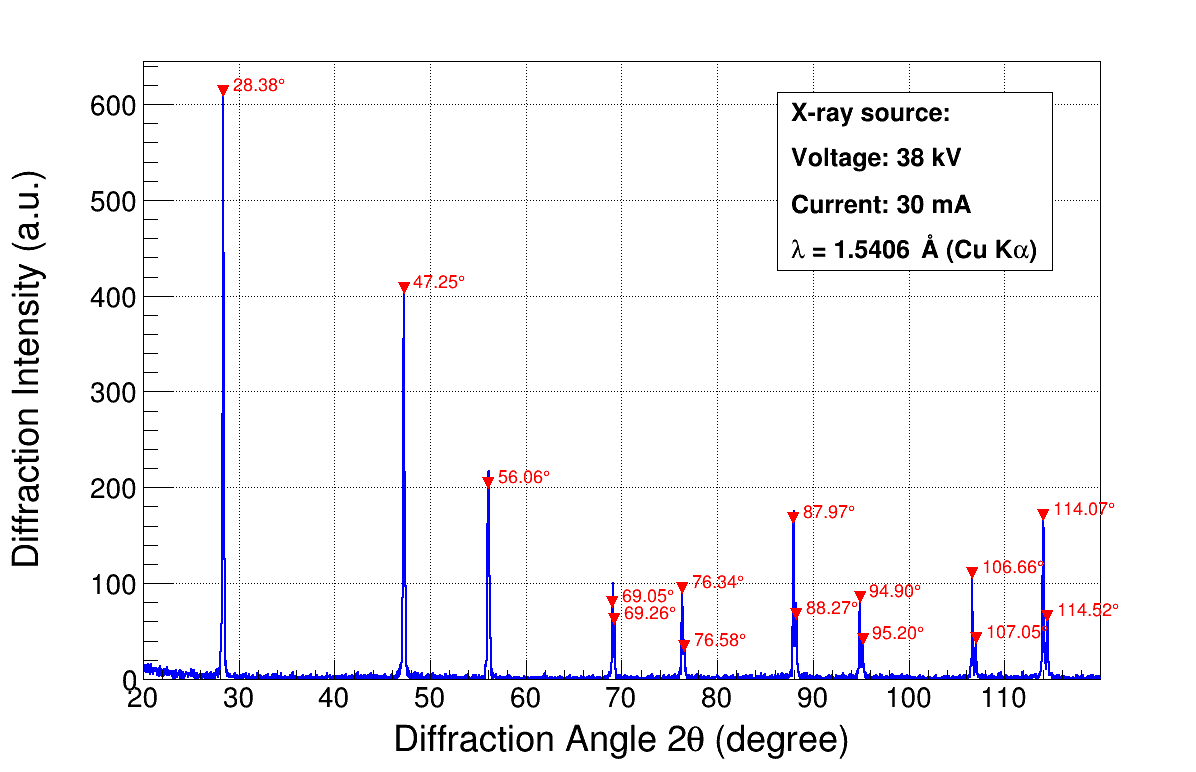
\includegraphics[options]{../Data/Silicon-multi.png}
    \caption{多晶硅粉末的X射线衍射谱图}
    \label{fig:si_xrd}    
\end{figure}

\begin{table}[H]
    \centering
    \captionnamefont{\wuhao\bf\heiti}
    \captiontitlefont{\wuhao\bf\heiti}
    \caption{多晶硅粉末X射线衍射谱寻峰结果表}
    \label{tab:si_xrd}
    \liuhao
    \begin{tabular}{ccccc}
        \toprule
        \midrule
        \bottomrule
    \end{tabular}
\end{table}

首先使用三强峰方法进行匹配以及比对:选取衍射强度最强的三个衍射峰,与PDF卡片中所载相对强度最大的衍射峰进行对比。通过Jade 9软件调取PDF#98-000-0396卡片进行对比,结果如下:

\begin{table}[H]
    \centering
    \captionnamefont{\wuhao\bf\heiti}
    \captiontitlefont{\wuhao\bf\heiti}
    \caption{多晶硅粉末X射线衍射谱三强峰法匹配结果表}
    \label{tab:si_xrd_tri_comp}
    \liuhao
    \begin{tabular}{ccccc}
        \toprule
        \midrule
        \bottomrule
    \end{tabular}
\end{table}

在以上几个衍射峰中,可以看到,衍射角度和相对强度符合得很好。进一步结合PDF卡片,标出其他衍射峰所对应晶面指数:

\begin{table}[H]
    \centering
    \captionnamefont{\wuhao\bf\heiti}
    \captiontitlefont{\wuhao\bf\heiti}
    \caption{多晶硅粉末X射线衍射峰晶面指数标定表}
    \label{tab:si_xrd_indexed}
    \liuhao
    \begin{tabular}{ccccc}
        \toprule
        \midrule
        \bottomrule
    \end{tabular}
\end{table}

所得各峰的位置与PDF卡片所载公认值符合很好,由此可以确认实验仪器以及分析方法可靠。

\subsubsection{关于多晶硅X射线“多重衍射峰”的讨论}

\subsubsection{Nelson-Reily外推法精确测定多晶硅样品晶格常数}

在X射线衍射实验中,样品以及转动台的偏心性、样品受X射线照射样品长度有限等因素都将对衍射角$\theta$测量值引入系统误差。结合Bragg公式(式\ref{eq:bragg}),将所使用的X射线波长$\lambda$视为完全确定,可以得到不确定度关系:

\begin{equation}
    \frac{\Delta d}{d} = \cot{\theta}\Delta\theta 
    \label{eqn:d_err}
\end{equation}

由此可以推知,对于$\theta$较大区域的衍射峰,由其测量得到的晶面间距所携带的相对误差较小,因而更有利于实现精密测量。

Taylor和Sinclair于1945年更进一步地提出,以上所述及的各项系统误差,若体现在晶格常数$a$测定值中,与衍射角$\theta$的关系可以用以下函数关系描述:

\begin{equation}
    \begin{cases}
        \frac{\Delta a}{a} & \propto f(\theta) \\
        f(\theta) & = \frac{1}{2} \left(\frac{\cos^2\theta}{\sin\theta} + \frac{\cos^2\theta}{\theta}\right) \\
    \end{cases}
\end{equation}

同年,Nelson和Riley使用$\text{Cu_9Al_4}$样品进行X射线晶体衍射实验,确认这一函数可以在$\theta > 30^\circ$范围内较好描述不同吸收度样品的系统误差。实际上,考虑到$f\left(\frac{\pi}{2}\right) = 0$,可以将各个衍射峰处测得的晶格常数$a$与相应衍射角$\theta$进行$a-f(\theta)$作图,并且进行线性外推,取$\theta=\frac{\pi}{2}$时外推值,即纵轴截距$a_0$作为实际测量值。此即Nelson-Reily外推法。

对多晶硅样品,借助于Nelson-Reily外推法,有如下外推结果:

\begin{table}[H]
    \centering
    \captionnamefont{\wuhao\bf\heiti}
    \captiontitlefont{\wuhao\bf\heiti}
    \caption{Nelson-Riley外推法测量硅晶体晶格常数数据表}
    \label{tab:si_xrd_extrapol}
    \liuhao
    \begin{tabular}{ccccc}
        \toprule
        \midrule
        \bottomrule
    \end{tabular}
\end{table}

表\ref{tab:si_xrd_extrapol}中给出的$a_0$的测量误差仅计入了外推的统计不确定度,这较于实际总不确定度仍偏小。即便如此,与PDF卡片所给参考值$a_0^{\text{Si, PDF}} = $的差值也已在不确定度范围内,进一步确认实验仪器以及分析方法可靠。

\subsection{}

\subsubsection{样品托架本底的排除}



\section{结论}


%%%%%%%%%%%%%%%%%%%%%%%%%%%%%%%%%%%%%%%%%%%%%%%%%%%%%%%%%%%%%%%%
%  参考文献
%%%%%%%%%%%%%%%%%%%%%%%%%%%%%%%%%%%%%%%%%%%%%%%%%%%%%%%%%%%%%%%%
%  参考文献按GB/T 7714-2015《文后参考文献著录规则》的要求著录. 
%  参考文献在正文中的引用方法:\cite{bib文件条目的第一行}

\renewcommand\refname{\heiti\wuhao\centerline{参考文献}\global\def\refname{参考文献}}
\vskip 12pt


\let\OLDthebibliography\thebibliography
\renewcommand\thebibliography[1]{
  \OLDthebibliography{#1}
  \setlength{\parskip}{0pt}
  \setlength{\itemsep}{0pt plus 0.3ex}
}

{
\renewcommand{\baselinestretch}{0.9}
\liuhao
\bibliographystyle{gbt7714-numerical}
\bibliography{./Report/TempExample}
}

\appendix
\section{衍射谱寻峰数据}


\end{document}
